\documentclass{beamer}

\input{../../spec_files/course_preamble.tex}
\subtitle{Foundations of Neuro-Symbolic AI}
\date{Summer Term 2026}
\author[FONS]{Alex Goessmann}
\institute[]{
    University of Applied Science Würzburg-Schweinfurt
%    Weierstrass Institute for Applied Analysis and Stochastic
}

%\newcommand{\techwstitle}{
%\small
%%Workshop \\
%Logik für Erklärbare KI:
%Technische Einführung in das ENEXA Projekt}
%\newcommand{\smalltechwstitle}{ENEXA Workshop}

%\newcommand{\techwsdate}{15.+16. July, 2024}

%\newcommand{\techwsauthors}{
%Alex Goessmann
%}

%\newcommand{\techwsinclude}{
%	\usepackage{../../spec/beamercolorthemeclaw}
%	\usepackage{/Users/alexgoessmann/Documents/ENEXA/latex_macros/beamer_template/beamerfontthemeclaw}
%	\usepackage{/Users/alexgoessmann/Documents/ENEXA/latex_macros/beamer_template/beamerinnerthemeclaw}
%	\usepackage{/Users/alexgoessmann/Documents/ENEXA/latex_macros/beamer_template/beamerouterthemeclaw}
%
%	\input{/Users/alexgoessmann/Documents/ENEXA/latex_macros/packages.tex}
%	\input{/Users/alexgoessmann/Documents/ENEXA/latex_macros/macros.tex}
%	\input{/Users/alexgoessmann/Documents/ENEXA/latex_macros/macros_tc.tex}
%	\input{/Users/alexgoessmann/Documents/ENEXA/latex_macros/tikz_blocks.tex}
%
%	\subtitle{\techwstitle}
%	\date[\techwsdate]{\techwsdate}
%	\author[\smalltechwstitle]{\techwsauthors}
%	\institute[]{\eupic}
%}

\newcommand{\techwschapterone}{I-Tensors}
\newcommand{\techwschaptertwo}{II-Probabilities}
\newcommand{\techwschapterthree}{III-Logics}
\newcommand{\techwschapterfour}{IV-Applications}

\newcommand{\eupic}{
\begin{center}
	%\includegraphics[width=4cm]{/Users/alexgoessmann/Documents/ENEXA/latex_macros/images/fundedEU.png}
\end{center}
}

\newcommand{\enexadateveublock}{
\begin{center}\begin{tikzpicture}
  	%\node [anchor=center] at (0,0) {\includegraphics[width = 1.5cm]{/Users/alexgoessmann/Documents/ENEXA/latex_macros/images/DATEV.png}};
	%\node [anchor=center] at (2.5,0.5) {\includegraphics[width = 3.5cm]{/Users/alexgoessmann/Documents/ENEXA/latex_macros/images/enexa.png}};
	%\node [anchor=center] at (2.55,-0.5) {\includegraphics[width = 3cm]{/Users/alexgoessmann/Documents/ENEXA/latex_macros/images/fundedEU.png}};
\end{tikzpicture}\end{center}
}


%% OLD
\newcommand{\aselectionvariable}{L}
\newcommand{\vselectionvariable}{L}
\newcommand{\fselectionvariable}{L}
\newcommand{\cselectionvariable}{L}
\newcommand{\individualorder}{n}
\newcommand{\variableof}[1]{\indvariableof{#1}}
\newcommand{\sindex}{s}
\newcommand{\pindex}{p}
\newcommand{\oindex}{o}
\newcommand{\exquery}{q}
%\newcommand{\datapointof}[1]{x^{#1}}
\newcommand{\atomicqueryof}[1]{g_{#1}}
\newcommand{\facsystem}{\shortcatvariables}
\newcommand{\margprobof}[1]{\probat{#1}}
\newcommand{\mlnprobabilityof}[1]{\expdistof{#1}}
%\newcommand{\oldenexadateveublock}{
%	\begin{center}
%	\begin{minipage}{0.2\textwidth}
%		\begin{center}
%			\includegraphics[width = 2.5cm]{images/DATEV.png}
%		\end{center}
%	\end{minipage}
%	\begin{minipage}{0.55\textwidth}
%		\begin{center}
%			\includegraphics[width=5.5cm]{images/enexa.png} \\
%			\includegraphics[width=5.5cm]{images/fundedEU.png} \\
%		\end{center}
%	\end{minipage}
%	\end{center}
%}

\title[Markov Logic Networks]{
	\techwschapterthree \\
	{\huge Markov Logic Networks}
}

\begin{document}


{\frame[plain]{\titlepage}}


\begin{frame}{From Logics to Probability}

Why is logical reasoning not enough?
\begin{itemize}
	\item Evidence is \emph{incomplete}: Not all conditions to rules might be known
	\item Evidence is \emph{uncertain}: There might be errors in the  data
\end{itemize}

\medskip

Enhancement of semantics (upgrade of epistemologic assumptions):
\begin{itemize}
	\item \emph{Logic}: Possible/impossible 
	\item \emph{Probability}: Numeric uncertainties beyond possible/impossible
\end{itemize}

\medskip 
\medskip

Judea Pearl in Probabilistic Reasoning in Intelligent Systems (1988):
\begin{center}
	\it Research [...] should bring together \emph{logics} aptitude for \emph{handling the visible} and \emph{probabilities} ability to \emph{summarize the invisible}. %p23 end of 1.4
\end{center}

\end{frame}



\begin{frame}{Tensors as a common framework}

\begin{columns}
	\column{0.5 \linewidth} \centering 
	\textbf{Propositional Logics} \\
	\medskip
	Representation of semantics by
		\[ \exformula: \atomstates \rightarrow [2] = \{0,1\} \]	
	Tensor Networks by formula compositions \\
	\medskip
	Contractions decide entailment by checking
		\[ \mathcal{C}(\{{\kb},\bencodingof{\exformula}\}\{\catvariableof{\exformula}\}) \parallel \onehotmapof{1} \]
	\column{0.5 \linewidth} \centering 
	\textbf{Probabilities} \\
	\medskip
	Representation of uncertainties by
		\[ \probtensor : \facstates \rightarrow [0,1] \]
	Tensor Networks by conditional independencies\\
	\medskip
	Contractions answer probabilistic queries
		\[ \probof{\catvariable} = \contractionof{\probtensor}{\catvariable} \]
\end{columns}

\end{frame}


\begin{frame}{Probabilistic Interpretations of Logics}

Uniform distribution of the models of $\exformula$ is a distribution
\begin{align*}
	\probtensor^{\exformula} = \frac{1}{\contractionof{\{\exformula\}}{\varnothing}} \exformula
\end{align*}
where $\exformula$ is a \emph{hard constraint}: 
States $\atomindices\in\atomstates$ with $\exformula(\atomindices)=0$ have vanishing probability. \\
\medskip
We build a \emph{soft constraint} by a weight $\weight\in\rr$ tuning the quotient of probabilities 
\begin{align*}
	\expof{\weight \cdot \exformula}(\atomindices) = \begin{cases}
	1 & \text{  if  } \exformula(\atomindices) = 0 \\
	\expof{\weight} &  \text{  if  } \exformula(\atomindices) = 1 \\
	\end{cases}
\end{align*}
and normate to get a probability tensor
\begin{align*}
	\probtensor^{(\exformula,\weight)} = \frac{1}{\contractionof{\{\expof{\weight\cdot \exformula}\}}{\varnothing}} \expof{\weight\cdot\exformula} \, .
\end{align*}

\end{frame}



\begin{frame}{Collection of weighted formulas}

\begin{definition}[Markov Logic Network]
	The \emph{Markov Logic Network} to as set of formulas $\formulaset$ weighted by $\weight: \formulaset \rightarrow \rr$ is the distribution
	\begin{align*}
		\probtensor^{(\formulaset, \weight)} = \frac{1}{\partitionfunctionof{\formulaset,\weight}}
		\contractionof{\expof{\weightof{\exformula}\cdot \exformula} \, : \, \exformulain}{\enumeratedatoms}
	\end{align*}
	where
	\begin{align*}
		\partitionfunctionof{\formulaset,\weight} = \contractionof{\left\{\expof{\weightof{\exformula}\cdot \exformula} \, : \, \exformulain\right\}}{\varnothing}
	\end{align*}
	is called the partition function.
\end{definition}

\end{frame}



%\begin{frame}{Tensor Calculus for Complex Sentences}
%
%\begin{block}{Representation of Complex Sentences}
%	The semantics of complex sentences are retrieved by \emph{contractions} of their connective semantics, which are summations of tensor coordinates among shared axes.
%	\begin{itemize}
%		\item Choose distributed representation to avoid contractions
%		\item Only execute those contractions required by reasoning 
%	\end{itemize}
%\end{block}
%
%Contractions can be depicted graphically by a \emph{Tensor Network}:
%\begin{center}
%	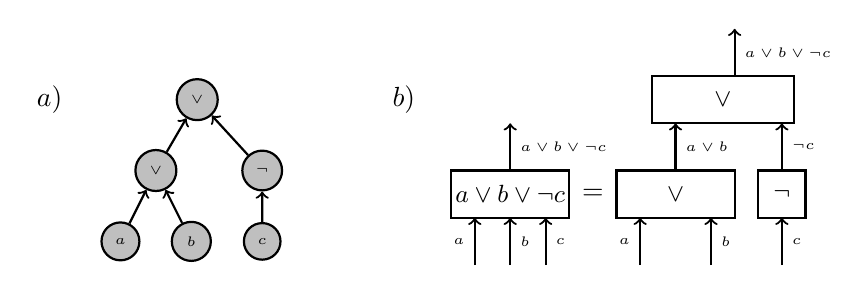
\begin{tikzpicture}[scale=0.3, yscale=-1, thick] % , baseline = -3.5pt

\begin{scope}[shift={(-15,0)}]

\node[anchor=center] (text) at (-3,-6) {${a)}$};

	\node [circle, draw, thick, fill=gray!50] (T1) at (0,0) {\tiny $a$};
	\node [circle, draw, thick, fill=gray!50] (T2) at (3,0) {\tiny $b$};
	\node [circle, draw, thick, fill=gray!50] (T3) at (6,0) {\tiny $c$};
	
	\node [circle, draw, thick, fill=gray!50] (and) at (1.5,-3) {\tiny $\lor$};
	\node [circle, draw, thick, fill=gray!50] (not) at (6,-3) {\tiny $\lnot$};	
	
	\draw [->] (T1) -- (and);
	\draw [->] (T2) -- (and);
	
	\draw [->] (T3) -- (not);	
	
	\node [circle, draw, thick, fill=gray!50] (head) at (3.25,-6) {\tiny $\lor$};
	
	\draw [->] (and) -- (head);
	\draw [->] (not) -- (head);			
\end{scope}

\node[anchor=center] (text) at (-3,-6) {${b)}$};

\draw[->] (0,1)--(0,-1) node[midway,left] {\tiny ${a}$}; 
\draw[->] (1.5,1)--(1.5,-1) node[midway,right] {\tiny ${b}$}; 
\draw[->] (3,1)--(3,-1) node[midway,right] {\tiny ${c}$}; 
\draw (-1,-1) rectangle (4, -3);
\node[anchor=center] (text) at (1.5,-2) {\small $\bencodingof{a \lor b \lor \lnot c}$};
\draw[->] (1.5,-3)--(1.5,-5) node[midway,right] {\tiny ${a \lor b \lor \lnot c}$}; 

\node[anchor=center] (text) at (5,-2) {${=}$};


\begin{scope}[shift={(7,0)}]

\draw[->] (0,1)--(0,-1) node[midway,left] {\tiny ${a}$}; 
\draw[->] (3,1)--(3,-1) node[midway,right] {\tiny ${b}$}; 
\draw[->] (6,1)--(6,-1) node[midway,right] {\tiny ${c}$}; 
	
\draw (-1,-1) rectangle (4, -3);
\node[anchor=center] (text) at (1.5,-2) {\small $\bencodingof{\lor}$};

\draw[->] (1.5,-3) --(1.5,-5) node[midway,right]{\tiny ${a \lor b}$};

\draw (5,-1) rectangle (7, -3);
\node[anchor=center] (text) at (6,-2) {\small $\bencodingof{\lnot}$};

\draw[->] (6,-3) --(6,-5) node[midway,right]{\tiny ${\lnot c}$};
	
\draw (0.5,-5) rectangle (6.5,-7);
\node[anchor=center] (text) at (3.5,-6) {\small $\bencodingof{\lor}$};
	
\draw[->] (4,-7) -- (4,-9) node[midway,right] {\tiny ${a \lor b \lor \lnot c}$};

%\draw (3,-9) rectangle (5,-11);
%\node[anchor=center] (text) at (4,-10) {$\truevectorat{}$};

\end{scope}

\end{tikzpicture}
%\end{center}
%
%\end{frame}




\begin{frame}{Tensor Network Representation}


Markov Logic Networks are represented by
\begin{itemize}
	\item 
\end{itemize}

\textbf{Markov Logic Networks combine logical and probabilistic approaches:}
\begin{itemize}
	\item Encoding of logical connectives are factors of the graphical model
	\item Further factors implement hard and soft constraints
\end{itemize}

\medskip

\textbf{Example:} Distribution over the atomic variables $a,b,c$ where
\begin{itemize}
	\only<1> {\item All worlds of equal probability ($\probtensor=\frac{1}{2^3}\ones$)}
	\only<2->{\item \textcolor{\concolor}{$ c \Rightarrow \big( a \lor b \big)$ is always true}}
	\only<3->{\item  \textcolor{\probcolor}{$a \lor b$ is likely to be true, tuned by a weight $\weightof{a \lor b}$}}
\end{itemize}

\begin{center}
	\begin{tikzpicture}[scale=0.35, thick, yscale=-1] % , baseline = -3.5pt


\draw[<-] (0,-1)--(0,1.5) node[below] {\tiny ${a}$}; 
\draw[<-] (1.5,-1)--(1.5,1.5) node[below] {\tiny ${b}$}; 
\draw[<-] (3,-1)--(3,1.5) node[below] {\tiny ${c}$}; 
\draw (-1,-1) rectangle (4, -3);
\node[anchor=center] (text) at (1.5,-2) {$\partitionfunction \cdot \probtensor$};



\node[anchor=center] (text) at (6.5,-2) {${=}$};


\begin{scope}[shift={(9,0)}]

\draw[->] (0,1)--(0,-1);%  node[midway,left] {\tiny ${a}$}; 
\draw (0,0.5)--(0,1.5) node[below] {\tiny ${a}$}; 
\draw[fill, \inactivecolor] (0,0.5) circle (0.25cm);
\draw[\inactivecolor] (0,0.5) -- (-0.5,0.5);
\draw[\inactivecolor]  (-2.5, 2.5) rectangle (-0.5, -0.5);
\node[anchor=center,\inactivecolor] (text) at (-1.5,1) {$\begin{bmatrix} 
1 \\
1
\end{bmatrix}$};

\draw[->]  (3,1)--(3,-1);% node[midway,right] {\tiny ${b}$}; 
\draw (3,0.5)--(3,1.5) node[below] {\tiny ${b}$}; 
\draw[fill, \inactivecolor] (3,0.5) circle (0.25cm);
\draw[\inactivecolor] (3,0.5) -- (2.5,0.5);
\draw[\inactivecolor]  (0.5, 2.5) rectangle (2.5, -0.5);
\node[anchor=center,\inactivecolor] (text) at (1.5,1) {$\begin{bmatrix} 
1 \\
1
\end{bmatrix}$};


\draw[->] (6,1)--(6,-1); % node[midway,right] {\tiny ${c}$}; 
\draw (6,0.5)--(6,1.5) node[below] {\tiny ${c}$}; 
\draw[fill, \inactivecolor] (6,0.5) circle (0.25cm);
\draw[\inactivecolor] (6,0.5) -- (5.5,0.5);
\draw[\inactivecolor]  (3.5, 2.5) rectangle (5.5, -0.5);
\node[anchor=center,\inactivecolor] (text) at (4.5,1) {$\begin{bmatrix} 
1 \\
1
\end{bmatrix}$};
	
\draw (-1,-1) rectangle (4, -3);
\node[anchor=center] (text) at (1.5,-2) {$\bencodingof{\lor}$};

\draw[->] (1.5,-3) --(1.5,-6) node[midway,right]{\tiny ${a \lor b}$};



\draw[fill, \probcolor] (1.5,-4.5) circle (0.25cm);
\draw[\probcolor] (1.5,-4.5) -- (-0.25,-4.5);
\draw[\probcolor]  (-6.75, -3.5) rectangle (-0.25, -6.5);
\node[anchor=center,\probcolor] (text) at (-3.5,-5) {$\begin{bmatrix} 
1 \\
\expof{\weightof{a\lor b}}
\end{bmatrix}$};


\draw (5,-1) rectangle (7, -3);
\node[anchor=center] (text) at (6,-2) {$\bencodingof{\lnot}$};

\draw[->] (6,-3) --(6,-6) node[midway,left]{\tiny ${\lnot c}$};
	
\draw[fill, \inactivecolor] (6,-4.5) circle (0.25cm);
\draw[\inactivecolor] (6,-4.5) -- (7.25,-4.5);
\draw[\inactivecolor]  (9.25, -3.5) rectangle (7.25, -6.5);
\node[anchor=center,\inactivecolor] (text) at (8.25,-5) {$\begin{bmatrix} 
1 \\
1
\end{bmatrix}$};
	
	
\draw (0.5,-6) rectangle (6.5,-8);
\node[anchor=center] (text) at (3.5,-7) {$\bencodingof{\lor}$};
	
\draw[->] (4,-8) -- (4,-11) node[midway,right] {\tiny ${a \lor b \lor \lnot c}$};

\draw[fill,\concolor] (4,-9.5) circle (0.25cm);
\draw[\concolor] (4,-9.5) -- (2.25,-9.5);
\draw[\concolor]  (0.25, -8.5) rectangle (2.25, -11.5);
\node[anchor=center,\concolor] (text) at (1.25,-10) {$\begin{bmatrix} 
0 \\
1
\end{bmatrix}$};

%\draw (3,-9) rectangle (5,-11);
%\node[anchor=center] (text) at (4,-10) {$\truevectorat{}$};

\end{scope}

\end{tikzpicture}
\end{center}


\end{frame}




\begin{frame}{Infering Markov Logic Networks}

	\textbf{Logical:} \emph{Model counts} by tensor network contractions
	\begin{itemize}
		\item Global contractions: \emph{Model-theoretic Entailment}
		\item Local contractions: \emph{Constraint Propagation} 
	\end{itemize}
	
	\textbf{Probabilistic:} \emph{Conditional probabilities} by tensor network contractions	
	\begin{itemize}
		\item Exact Inference: \emph{Belief Propagation}
		\item Approximate Inference: \emph{Gibbs Sampling}, \emph{Loopy Belief Propagation}
	\end{itemize}

\begin{block}{Tradeoff}
	The size of tensor network contractions is a tradeoff between
	\begin{center}
		Completeness/Exactness  $\leftrightarrow$  Efficiency (Demand of the contraction)
	\end{center}
\end{block}

\end{frame}




\begin{frame}{Application of Markov Logic Networks}

(Ante-hoc \& globally) \emph{Explainable Generative Models} 
\begin{itemize}
	\item Human-machine interface based on interpretable logical sentences
	\item Expert evaluation and manipulation of models
	\item Generation of synthetic data (e.g. for test purposes)
\end{itemize}
\ \\ \ \\
\emph{Logic and Probabilistic Programming}
\begin{itemize}
	\item Generation by declarative programming or learned from data
	\item Prediction of unseen variables given evidence
	\item Explainability built-in by logics
	\item Uncertainty assessment built-in by probabilities
\end{itemize}
\ \\ \ \\
%Generation of \emph{Synthetic Data}
%\begin{itemize}
%	\item Structured generation of synthetic data
%	\item No privacy restriction apply
%\end{itemize}
	
\end{frame}



\begin{frame}{Implementation in \tnreason: \\
Subpackage \spapplication{}}

The subpackage \spapplication{} implements generalizations of Markov Logic Networks and corresponding reasoning tasks.

\begin{center}
\begin{tikzpicture}[scale=0.27]

\draw[dashed] (-30,15) -- (12,15) -- (12,-3) -- (-30,-3) -- (-30,15);

\draw[blue] (-10,10) rectangle (10,14); 
\node [blue, anchor=center] at (0,12) {\spapplication{}};

\node [anchor=center,blue] at (-20,12) {\layerthreespec};
\draw[dashed] (-30,9) -- (12,9);
\node [anchor=center] at (-20,6) {\layertwospec};

\draw[blue,->] (6,10) -- (6,8);
\draw[] (2,4) rectangle (10,8); 
\node [anchor=center] at (6,6) {\spreasoning{}};
\draw[->] (6,4) -- (6,2);

\draw[blue,->] (-6,10) -- (-6,8);
\draw[] (-10,4) rectangle (-2,8); 
\node [anchor=center] at (-6,6) {\sprepresentation{}};
\draw[->] (-6,4) -- (-6,2);

\draw[dashed] (-30,3) -- (12,3);
\node [anchor=center] at (-20,0) {\layeronespec};

\draw (-10,-2) rectangle (10,2); 
\node [anchor=center] at (0,0) {\spengine};
\end{tikzpicture}
\end{center}

\end{frame}


\begin{frame}{Extension of Script Language $\sencodingof{\cdot}$}

Formulas with hard logical interpretation are stored as before in \emph{fact dictionaries}:
\begin{centeredscript}
	\{key($\exformula$) : $\sencodingof{\exformula}$ for $\exformula\in\formulaset$\}
\end{centeredscript}

\medskip

Formulas with soft logical interpretation (as in Markov Logic Networks) are stored in \emph{weighted formulas dictionaries}:
\begin{centeredscript}
	\{key($\exformula$) : $\sencodingof{\exformula}$ + [$\weightof{\exformula}$] for $\exformula\in\formulaset$\}
\end{centeredscript}

\end{frame}


\begin{frame}{Hybrid Knowledge Bases}

Probability distributions, which are specified by propositional formulas are captured by the class
\begin{centeredscript}
	knowledge.HybridKnowledgeBase
\end{centeredscript}
initialized with arguments
\begin{itemize}
	\item \emph{facts:} Dictionary of propositional formulas stored as $\sencodingof{\exformula}$ representing hard logical constraints
	\item \emph{weightedFormulas:} Dictionary of propositional formulas stored as $\sencodingof{\exformula}$+$[\weightof{\exformula}]$ representing soft logical constraints
	\item \emph{evidence:} Dictionary of atomic formulas, where key are the formulas in string representation and values the certainty in $[0,1]$ (float or int) of the atom being true
	\item \emph{categoricalConstraints:} Dictionary of categorical constrained, which values are lists of atomic formulas stored as strings $\sencodingof{\atomicformula}$
\end{itemize}

\end{frame}


%\begin{frame}{Semantics of }
%
%Connective Cores are created to represent all required formulas
%
%Generic head cores:
%\begin{itemize}
%	\item $\onehotmapof{1}$ for hard constraints
%	\item $[1 \, \expof{\weight}]$ for soft constraints
%\end{itemize}
%
%Both in 
%\begin{centeredscript}
%	knowledge.HybridKnowledgeBase()
%\end{centeredscript}
%
%\end{frame}



\end{document}